\subsection{Sviluppo}
\subsubsection{Obiettivi}
Il processo di Sviluppo coinvolge tutte le attività volte alla produzione del prodotto finale: analisi dei requisiti,  progettazione, codifica, integrazione, testing e installazione. In particolar modo, questo processo viene istanziato con i seguenti obiettivi:
\begin{itemize}
	\item definizione dei vincoli e dei requisiti del sistema finale in accordo con i bisogni espressi dagli \textit{stakeholders\glo} in causa;
	\item scomposizione e classificazione dei requisiti coinvolti;
	\item studio e analisi delle tecnologie coinvolte durante la realizzazione del sistema;
	\item realizzazione di una progettazione (architetturale e di dettaglio) basata sull'utilizzo di \textit{design pattern\glo} consolidati;
	\item implementazione del prodotto che soddisfi i requisiti esposti dal proponente e dal committente e le convenzioni stabilite all'interno del team.
\end{itemize}
\subsubsection{Attività}
\paragraph{Analisi dei requisiti}
L'analisi dei requisiti comprende la descrizione dettagliata delle specifiche del sistema. È compito dell'analista descrivere, oltre che i requisiti funzionali del prodotto, anche quelli prestazionali, di qualità e di vincolo.
Questa attività ha come obiettivo il perseguimento delle seguenti caratteristiche:
\begin{itemize}
	\item \textbf{Chiarezza strutturale:} i requisiti devono essere classificati e organizzati in maniera precisa, distinguendo i requisiti funzionali da quelli non funzionali;
	\item \textbf{Chiarezza espressiva:} è necessario avere una chiarezza espositiva tale da permettere la definizione di requisiti non ambigui;
	\item \textbf{Atomicità dei requisiti:} occorre analizzare i bisogni fino a ché non si raggiungono requisiti atomici, non ulteriormente suddivisibili.
\end{itemize}

\subparagraph*{Requisiti}
L'approccio utilizzato per la definizione dei requisiti è stato di tipo \textbf{top-down}: il prodotto finale, a partire dalla sua totalità, è stato scomposto nelle parti che lo compongono sino ad arrivare a requisiti atomici. Le proprietà fondamentali di un requisito sono le seguenti:
\begin{itemize}
	\item devono essere verificabili;
	\item devono soddisfare tutti i bisogni espressi dall'utente;
	\item non devono soddisfare caratteristiche superflue (solo quelle strettamente necessarie);
	\item non devono essere contraddittori;
	\item devono essere tracciabili e modificabili.
\end{itemize}
\noindent Ogni requisito necessità tracciabilità. Verrà dunque utilizzato per ciascuno un codice identificativo strutturato nel seguente modo:
\\\\
\centerline{\textbf{[Priorità][Tipologia][Codice]}}\\
\begin{itemize}
  \item \textbf{Priorità}:
  \begin{itemize}
    \item \textbf{1 (Obbligatorio)}: necessario per almeno uno degli \textit{stakeholder\glos};
    \item \textbf{2 (Desiderabile)}: non strettamente necessario, ma di valore aggiunto;
    \item \textbf{3 (Opzionale)}: relativamente utili e contrattabili con l'avanzare del progetto.
  \end{itemize}
  \item \textbf{Tipologia}:
  \begin{itemize}
    \item \textbf{F:} funzionali;
    \item \textbf{P:} prestazionali;
    \item \textbf{Q:} qualitativi;
    \item \textbf{V:} di vincolo.
  \end{itemize}
  \item \textbf{Codice identificativo}.
\end{itemize}
Ogni requisito è opportunamente seguito da:
\begin{itemize}
  \item \textbf{Descrizione}: breve descrizione riguardante il requisito;
  \item \textbf{Fonte}: da dove proviene il requisito, chi l'ha richiesto o dove è stato ricavato. Le fonti di un requisito potranno essere le seguenti:
  \begin{itemize}
  	\item \textbf{Capitolato\glos:} se riportato nel \textit{capitolato\glos};
  	\item \textbf{Interna:} se concordato all'interno del team;
  	\item \textbf{Caso d'uso:} se derivato da un caso d'uso (verrà riportato il codice identificativo del caso d'uso come descritto nella sezione \textsection2.2.2.2);
  	\item \textbf{Verbale:} se concordato durante una riunione, verrà riportato il codice identificativo della decisione alla quale viene fatto riferimento.
  \end{itemize}
\end{itemize}

\subparagraph*{Casi d'uso}
I casi d'uso descrivono l'insieme delle casistiche con cui il sistema si interfaccia verso l'esterno. Ogni caso d'uso sarà identificato univocamente da un codice formato da:
\\\\
\centerline{\textbf{UC[Codicepadre].[Codicefiglio]}}\\

\begin{itemize}
	\item \textbf{Codicepadre:} identificativo numerico dato al caso d'uso a cui questo è associato;
	\item \textbf{Codicefiglio:} identificativo numerico per il sotto-caso corrente.
\end{itemize}
Ogni caso d'uso, oltre ad avere un relativo diagramma, verrà descritto
\begin{itemize}
  \item codice;
  \item nome;
  \item diagramma del caso d'uso;
  \item attori principali;
  \item attori secondari (opzionale);
  \item pre-condizioni;
  \item post-condizioni;
  \item scenario principale;
  \item inclusioni (opzionale);
  \item esclusioni (opzionale);
  \item specializzazioni (opzionale).
\end{itemize}

\subparagraph*{UML\glo}
Il gruppo Tenners utilizzerà la versione del linguaggio \textit{UML\glo} 2.0 per la realizzazione dei diagrammi dei casi d'uso.
\paragraph{Progettazione}
La progettazione è un'attività che si attiva al termine dell'analisi dei requisiti, ponendo le basi per l'implementazione effettiva del prodotto software. Lo scopo dei progettisti è capire come risolvere il problema di partenza e soddisfare i requisiti in modo ottimale. Diversamente da ciò che accade nell'analisi dei requisiti, in cui il problema viene progressivamente decomposto in parti più piccole, in questa attività si ricompone il tutto per definire la soluzione migliore. Si possono catalogare due tipologie di progettazione:
\begin{itemize}
	\item \textbf{progettazione architetturale:} progettazione di alto livello che descrive come il sistema deve essere organizzato nelle sue componenti;
	\item \textbf{progettazione di dettaglio:} descrive il comportamento delle singole componenti (e delle unità che le compongono) e il modo di interagire tra esse.
\end{itemize}
Nel contesto del progetto didattico, sono state stabilite due \textit{milestone}\glo distinte:
\begin{itemize}
	\item \textbf{Technology Baseline\glos}: Selezione delle tecnologie, \textit{framework}\glo e librerie tramite \textit{Proof of Concept (PoC)\glos}. Il \textit{PoC\glo} deve essere accessibile su \textit{GitHub\glos};
	\item \textbf{Product Baseline)\glos}: viene presentata una \textit{baseline\glo} architetturale coerente con quanto mostrato in Technology \textit{Baseline\glos}.
\end{itemize}
\subparagraph*{Technology Baseline\glo}
Ha lo scopo di:
\begin{itemize}
	\item motivare l'utilizzo di determinate tecnologie, \textit{framework\glo} e librerie;
	\item presentare un \textit{PoC\glo} eseguibile che venga utilizzato come \textit{baseline\glo} per l'attività di sviluppo;
	\item il codice del \textit{PoC\glo} non sarà usa e getta ma diverrà utile e necessario per i successivi incrementi del modello di sviluppo.
\end{itemize}
\subparagraph*{Product Baseline\glo}
Ha lo scopo di:
\begin{itemize}
	\item presentare la \textit{baseline\glo} architetturale del prodotto;
	\item illustrare tramite un allegato tecnico i diagrammi delle classi, di sequenza e i design pattern utilizzati contestualizzati all'architettura.
\end{itemize}
\subparagraph*{Architettura}
Il gruppo ha deciso di garantire una buona architettura perseguendo i seguenti obiettivi qualitativi:
\begin{itemize}
	\item \textbf{sufficienza:} deve soddisfare tutti i requisiti rilevati nella precedente attività di analisi;
	\item \textbf{comprensibilità:} deve poter essere compresa da tutti gli \textit{stakeholders\glo} coinvolti;
	\item \textbf{modularità:} suddivisione in parti non sovrapponibili tra loro e ben distinte;
	\item \textbf{robustezza:} gestione di un'ampia tipologia di input. Qualità strettamente legata alla modularità dell'architettura;
	\item \textbf{flessibilità:} capacità dell'architettura di evolversi e cambiare, a costi contenuti, al variare dei requisiti;
	\item \textbf{efficienza:} spreca il meno possibile in termini di spazio, tempo;
	\item \textbf{affidabilità:} esegue quello che ci si aspetta nella maniera corretta;
	\item \textbf{disponibilità:} in caso di manutenzione, il sistema rimarrà indisponibile senza aver un impatto importante sull'utenza;
	\item \textbf{sicurezza:} l'architettura non deve essere vulnerabile a intrusioni e, in caso di eventuali malfunzionamenti, deve essere garantito il funzionamento delle restanti parti dell'architettura;
	\item \textbf{semplicità:} deve soddisfare i soli requisiti necessari, eliminando funzionalità superflue;
	\item \textbf{incapsulamento:} necessità di nascondere lo stato interno esponendo solo ciò che è necessario sapere;
	\item \textbf{coesione:} presenza di coesione funzionale, sequenziale e informativa tra le componenti che costituiscono i moduli dell'architettura;
	\item \textbf{basso accoppiamento:} le componenti dell'architettura devono dipendere il meno possibile l'una dall'altra.
\end{itemize}

\subparagraph*{Diagrammi di sequenza} Descrivono uno scenario composto da una sequenza di azioni le cui scelte sono già state effettuate. Non ammette dunque flussi alternativi. Il diagramma si sviluppa su linee verticali parallele che rappresentano l'avanzare del tempo. Esso è costituito da:
\begin{itemize}
	\item \textbf{partecipanti:} entità che comunicano tra di loro;
	\item \textbf{messaggi:} dati e operazioni che vengono scambiati tra i partecipanti. Essi possono essere di diverse tipologie:
	\begin{itemize}
		\item sincroni;
		\item asincroni;
		\item di ritorno;
		\item creazione;
		\item distruzione
	\begin{figure}[h!]
		\caption{Tipologie di messaggi in un diagramma di sequenza}
		\centering
		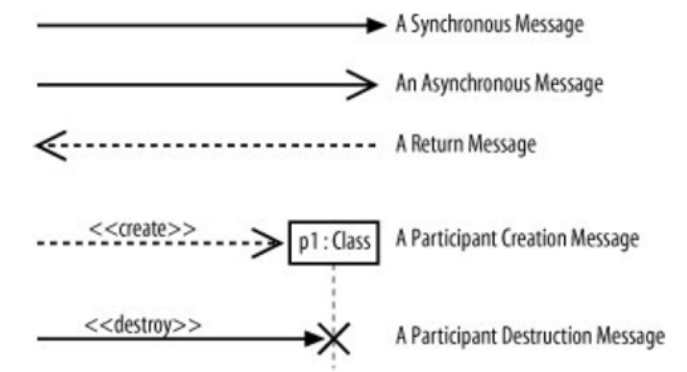
\includegraphics[width=\textwidth]{res/img/diagrammiDiSequenza.png}
	\end{figure}
	\end{itemize}
	\item \textbf{barra di attivazione:} rettangolo, posizionato sulla linea della vita di un partecipante, che ne indica il periodo di attività.
\end{itemize}

\subparagraph*{Diagrammi delle classi} Descrivono il tipo di oggetti che fanno parte di un sistema e le relazioni che intercorrono tra loro. La descrizione delle classi dovrà essere così strutturata:
\begin{itemize}
	\item \textbf{nome della classe (obbligatorio)}
	\item \textbf{attributi (feature):} Rappresentano i membri della classe. Saranno descritti nel seguente modo: \\\\ \centerline{\textbf {visibilità nome : tipo [molteplicità] = default [proprietà aggiuntive]}}\\
	\begin{itemize}
		\item visibilità:
		\begin{itemize}
			\item (+) public;
			\item (\#) protected;
			\item (~) package;
			\item (-) private.
		\end{itemize}
	\end{itemize}
	\item \textbf{operazioni (feature):} Servizi che possono essere richiesti quando si istanzierà un oggetto della classe. Saranno descritti nel seguente modo: \\\\ \centerline{\textbf {visibilità nome (lista-parametri) : tipo-ritorno [proprietà aggiuntive]}}\\\\
	dove:
	\\\\ \centerline{\textbf {lista-parametri := direzione nome : tipo = default}}\\
	\begin{itemize}
		\item visibilità:
		\begin{itemize}
			\item (+) public;
			\item (\#) protected;
			\item (~) package;
			\item (-) private.
		\end{itemize}
		\item direzione:
		\begin{itemize}
			\item in;
			\item out;
			\item in-out;
		\end{itemize}
	\end{itemize}
\end{itemize}
\noindent Tra le classi possono sussistere delle relazioni può o meno costrittive. Per raffigurarne il grado di dipendenza, vengono utilizzate le seguenti tipologie di frecce:
\begin{figure}[h!]
	\caption{Raffigurazione delle relazioni tra classi}
	\centering
	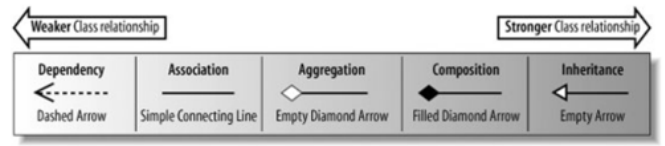
\includegraphics[width=0.8\textwidth]{res/img/relazioniClassi.png}
\end{figure}
\begin{itemize}
	\item \textbf{dipendenza:} indica una relazione breve tra gli oggetti di una classe con quelli di un'altra. Questa tipologia di relazione si verifica in due situazioni:
	\begin{itemize}
		\item un metodo di una classe "A" riceve come parametro una istanza di un'altra classe "B";
		\item la classe "A" crea un oggetto di tipo "B" in uno dei suoi metodi.
	\end{itemize}
	\item \textbf{associazione:} quando un oggetto di una classe lavora con oggetti di altre classi per un periodo prolungato. Tale relazione si verifica ad esempio nel caso in cui un attributo di una classe "A" e di tipo "B". Sarà necessario dunque, ad ogni costruzione di un oggetto di "A", costruire anche l'oggetto di tipo "B";
	\item \textbf{aggregazione:}  quando una classe possiede ma condivide un riferimento ad oggetti di
	un’altra classe. Indica, in altre parole, una relazione di tipo "parte di..";
	\item \textbf{composizione:} quando una classe "A" contiene oggetti di un’altra classe "B". In questo caso gli oggetti di tipo "B" non possono esistere senza il contenitore (tipo "A");
	\item \textbf{ereditarietà:} quando si instaurano relazioni di sottotipaggio.
\end{itemize}

\subparagraph*{Diagrammi di oggetti} Descrivono il sistema mediante gli oggetti e le associazioni tra loro. Seguono il modello descritto dai diagrammi delle classi, senza però avere alcun elemento obbligatorio. Tramite questi diagrammi è possibile inoltre verificare i valori delle proprietà associate ad un oggetto.

\subparagraph*{Diagrammi dei package} Documentano la dipendenza tra classi. Essi avranno le seguenti caratteristiche:
\begin{itemize}
	\item ogni package è caratterizzato da una etichetta che ne specifica il nome;
	\item ogni classe all'interno di un package è caratterizzata dalla visibilità che possiede nei confronti degli altri package (pubblica o privata);
\end{itemize}

\subparagraph*{Diagrammi di attività} Descrivono la logica procedurale che compone un processo. Essi sono composti da:
\begin{itemize}
	\item \textbf{nodo iniziale:} punto da cui inizia il processo;
	\item \textbf{nodo finale:} punto in cui termina il processo;
	\item \textbf{fork:} elaborazione parallela di più processi;
	\item \textbf{join:} sincronizzazione rispetto ad una determinata condizione di processi che sino a quel momento eseguivano in parallelo;
	\item \textbf{branch:} rami decisionali in cui si può intraprendere uno solo dei percorsi a disposizione.
\end{itemize}


%\subparagraph*{Diagrammi per la Progettazione}
%Per facilitare la descrizione dell'architettura del prodotto finale, si ricorre all'utilizzo di alcune tipologie di diagrammi \textit{UML\glos}:
%\begin{itemize}
%	\item \textbf{Diagrammi di sequenza:} descrivono uno scenario composto da una sequenza di azioni le cui scelte sono già state effettuate. Non ammette dunque flussi alternativi;
%	\item \textbf{Diagrammi delle classi:} descrivono il tipo di oggetti che fanno parte di un sistema;
%	\item \textbf{Diagrammi dei package:} documentano la dipendenza tra classi;
%	\item \textbf{Diagrammi di attività:} descrivono la logica procedurale che compone un processo;
%	\item \textbf{Diagrammi di oggetti:} descrivono il sistema mediante gli oggetti e le associazioni tra loro.
%\end{itemize}
\paragraph{Codifica}
Durante la Codifica viene sviluppato il codice del prodotto software dai programmatori. È fondamentale che questo risulti uniforme per migliorarne le attività di manutenzione, verifica e validazione. È quindi necessario normare il lavoro in modo tale che il loro codice risulti leggibile, attraverso uno stile di codifica.
\subparagraph*{Stile di codifica}
Stabilire convenzioni di codifica comuni, migliora la leggibilità del codice e lo rende più facilmente mantenibile. Il gruppo Tenners, per aumentare l'omogeneità e l'uniformità durante la stesura del codice richiesta da \textit{capitolato\glos}, ha scelto delle regole comuni da seguire derivanti dallo stile di codifica dettato da eslint-airbnb:
\begin{itemize}
  \item \textbf{Indentazione}: per l'indentazione dei blocchi saranno utilizzati 2 caratteri spazio (e non il classico tab), per uniformare la codifica dei caratteri su diversi sistemi operativi;
  \item \textbf{Posizione delle parentesi}: le parentesi per l'apertura di un blocco vanno inserite in linea con i costrutti mentre, quelle di chiusura, vanno inserite alla linea successiva rispetto all'ultima istruzione del blocco.
  Esempio:
  \begin{lstlisting}
  	function toCelsius(fahrenheit) {
  		return (5 / 9) * (fahrenheit - 32);
  	}
  \end{lstlisting}
  \item \textbf{Nomenclatura}: i nomi contenuti nel codice devono aderire alle seguenti convenzioni:
  \begin{itemize}
  	\item \textbf{Nome delle classi:} scritti in UpperCamelCase, senza l'utilizzo degli spazi, con la prima lettera di ciascuna parola in maiuscolo Esempio:
  	\begin{lstlisting}
  	class AccountingDepartment {
  		....
  	}
  	\end{lstlisting}
  	\item \textbf{Nome dei metodi e delle variabili:} scritti in lowerCamelCase, senza l'utilizzo degli spazi, con la prima lettera di ciascuna parola in maiuscolo eccetto la prima. Il loro nome di deve suggerire l'azione eseguita. Esempio:
  	\begin{lstlisting}
  	let z = 100;
  	function addToZ(x, y) {
  		return x + y + z;
  	}
  	\end{lstlisting}
  \end{itemize}
  Per facilitare la lettura e la comprensione del codice, tutti i nomi devono essere significativi e parlanti;
  \item \textbf{Lingua}: il codice e i commenti vanno scritti in lingua inglese;
  \item \textbf{Spazi intorno agli operatori:} verranno inseriti degli spazi intorno agli operatori ( = + - * / ) , e dopo le virgole.
  Esempio:
  \begin{lstlisting}
  var x = y + z;
  var values = [ 'Volvo', 'Saab', 'Fiat' ];
  \end{lstlisting}

\end{itemize}
%\subparagraph{TypeScript}

\subsubsection{Strumenti}
\paragraph{Visual Paradigm 13 CE}
Software utilizzato per la stesura dei diagrammi dei casi d'uso, delle classi e dei package. Permette una gestione semplice degli elementi del diagramma tramite semplici drag and drop e la versione Community Edition è disponibile gratuitamente e dunque accessibile a tutti i membri del gruppo.

\paragraph{AWS Lambda}
Servizio che consente di eseguire codice nel \textit{cloud}\glos. Esso viene utilizzato per la componente \textit{etherless-server}.

\paragraph{Visual Studio Code}
Visual Studio Code è un editor di codice sorgente che supporta, tra gli altri, il linguaggio Typescript. Tale software viene imposto dal \textit{capitolato\glos}.

\paragraph{Ethereum\glo}
Rete globale per il trasferimento di \textit{criptovalute}\glo e per la realizzazione di applicativi decentralizzati.

\paragraph{Truffle}
Framework per lo sviluppo di \textit{smart contract\glo} su rete \textit{Ethereum\glo}s.

\paragraph{Smart contract\glo}
Protocollo informatico che facilita, verifica, fa rispettare ed esegue un
contratto (insieme di regole).

\paragraph{Ropsten}
Rete \textit{Ethereum}\glo pubblica usato per il testing di applicativi \textit{Ethereum\glo} prima
del \textit{porting\glo} in produzione sulla \textit{MainNet\glos}.

\paragraph{AWS Elastic Beanstalk}
Sevizio offerto dalla piattaforma di AWS. Utilizzato per tenere in esecuzione continua la componente "Runner" e rimanere in costante ascolto degli eventi emessi dalla rete \textit{Ethereum\glo}.

\newpage \subsubsection{Linguaggi}
\paragraph{Typescript 3.6}
Versione standardizzata da Microsoft del linguaggio JavaScript.

\paragraph{Node.js}
Ambiente di runtime \textit{open-source}\glo per JavaScript.

\paragraph{Serverless\glo Framework\glo}
Framework\glo per la costruzione di ambienti serverless\glos e, in particolare, per la creazione di applicazioni su AWS Lambda.

\paragraph{Solidity}
Linguaggio OOPG per la definizione di \textit{smart contract}\glos.

\paragraph{Web3}
\textit{API}\glo JavaScript per l’interazione con un nodo \textit{Ethereum\glos}, locale o remoto.\\

 

\subsubsection{Procedure}
\paragraph{Visual Paradigm - Salvataggio diagramma dei casi d'uso}
\begin{enumerate}
	\item Cliccare sulla finestra "Project";
	\item Cliccare sul bottone "Export;
	\item Cliccare su "XML...";
	\item Selezionare tutti i diagrammi utilizzati tramite le checkbox;
	\item Selezionare il percorso di destinazione;
	\item Cliccare su "Export".
\end{enumerate}

\paragraph{Visual Paradigm - Caricamento diagramma dei casi d'uso}
\begin{enumerate}
	\item Cliccare sulla finestra "Project";
	\item Cliccare sul bottone "Import;
	\item Cliccare su "XML...";
	\item Digitare il percorso del file con estensione .XML;
	\item Cliccare su "Import".
\end{enumerate}
